\documentclass[xetex,mathserif,serif]{beamer}

\usepackage{xunicode}
\usepackage{xltxtra}
\usepackage{color}
\usepackage{url}
\usepackage{listings}
\usepackage{fontspec}
\usepackage{geometry}
\usepackage{lastpage}
\usepackage{fancyhdr}
\usepackage{amsmath}
\usepackage{amsthm}
\usepackage{amssymb}
\usepackage{blkarray}
\usepackage{multicol}
\usepackage{relsize}

\definecolor{solarized@base03}{HTML}{002B36}
\definecolor{solarized@base02}{HTML}{073642}
\definecolor{solarized@base01}{HTML}{586e75}
\definecolor{solarized@base00}{HTML}{657b83}
\definecolor{solarized@base0}{HTML}{839496}
\definecolor{solarized@base1}{HTML}{93a1a1}
\definecolor{solarized@base2}{HTML}{EEE8D5}
\definecolor{solarized@base3}{HTML}{FDF6E3}
\definecolor{solarized@yellow}{HTML}{B58900}
\definecolor{solarized@orange}{HTML}{CB4B16}
\definecolor{solarized@red}{HTML}{DC322F}
\definecolor{solarized@magenta}{HTML}{D33682}
\definecolor{solarized@violet}{HTML}{6C71C4}
\definecolor{solarized@blue}{HTML}{268BD2}
\definecolor{solarized@cyan}{HTML}{2AA198}
\definecolor{solarized@green}{HTML}{859900}
\definecolor{yaleblue}{HTML}{0E4C92}

\newcommand{\yellow}[1]{\textcolor{solarized@yellow}{#1}}
\newcommand{\orange}[1]{\textcolor{solarized@orange}{#1}}
\newcommand{\red}[1]{\textcolor{solarized@red}{#1}}
\newcommand{\magenta}[1]{\textcolor{solarized@magenta}{#1}}
\newcommand{\violet}[1]{\textcolor{solarized@violet}{#1}}
\newcommand{\blue}[1]{\textcolor{solarized@blue}{#1}}
\newcommand{\cyan}[1]{\textcolor{solarized@cyan}{#1}}
\newcommand{\green}[1]{\textcolor{solarized@green}{#1}}
\newcommand{\yblue}[1]{\textcolor{yaleblue}{#1}}

\setbeamertemplate{navigation symbols}{}
% \setbeamerfont{title}{family=\old}
% \setbeamerfont{author}{family=\tfont}%
% \setbeamerfont{frametitle}{family=\oldA}
% \setbeamerfont{date}{family=\dfont}

% \addtobeamertemplate{navigation symbols}{}{%
%     \usebeamerfont{footline}%
%     \usebeamercolor[fg]{footline}%
%     \hspace{1em}%
%     \insertframenumber/\inserttotalframenumber
% }

\setbeamertemplate{footline}[text line]{%
  \parbox{0.99\linewidth}{
    \normalsize\vspace*{-24pt}\hfill{\color{solarized@base00}\insertframenumber/\inserttotalframenumber}
  }
}


\setbeamertemplate{itemize items}{--}
\setbeamercolor*{item}{fg=black}

\defaultfontfeatures{Mapping=tex-text}
\hypersetup{pdfstartview={FitH}}

\newcommand{\old}[1]{\fontspec[Alternate=1,Ligatures={Common}]{Hoefler Text}\fontsize{18pt}{30pt}\selectfont #1}%
\newcommand{\oldA}[1]{\fontspec[Alternate=1,Ligatures={Common, Rare}]{Hoefler Text}\fontsize{12pt}{15pt}\selectfont #1}%
\newcommand{\oldB}[1]{\fontspec[Ligatures={Common}]{Didot}\fontsize{12pt}{15pt}\color{solarized@base02}\selectfont #1}%
\newcommand{\tfont}[1]{\fontspec[Alternate=1,Ligatures={Common}]{Hoefler Text}\fontsize{12pt}{20pt}\selectfont #1}%
\newcommand{\dfont}[1]{\fontspec[Ligatures={Common}]{Didot}\fontsize{12pt}{12pt}\selectfont #1}%

% \newcommand{\minimize}{\mathop{\mathrm{minimize}}}
\newcommand{\argmin}{\mathop{\mathrm{arg\,min}}}
\newcommand{\argmax}{\mathop{\mathrm{arg\,max}}}
\newcommand{\st}{\mathop{\mathrm{subject\,\,to}}}

\newcommand\independent{\protect\mathpalette{\protect\independenT}{\perp}}
\def\independenT#1#2{\mathrel{\rlap{$#1#2$}\mkern2mu{#1#2}}}

\setlength{\parindent}{0pt}
\setlength{\parskip}{12pt}

\setromanfont [Ligatures={Common}, Numbers={OldStyle}, Variant=01,
 BoldFont={LinLibertine_RB.otf},
 ItalicFont={LinLibertine_RI.otf},
 BoldItalicFont={LinLibertine_RBI.otf}
 ]{LinLibertine_R.otf}



\usepackage{sty/personalmacros}
\usepackage{sty/personalslides}

\begin{document}
%%%%%%%%%%%%%%%%%%%%%%%%%%%%%%%%%%%%%%%%%%%%%%%%%%%%%%%%%%%%%%%%%%%%%%%%%%%%%%%
% Manifest
% --------
% - Title
% - Outline
% - Review of Graphical Models
% - Review of Multivariate Gaussian
% - Precision Matrices in Context of Gaussian Graphical Models
% - Pairwise Inference for Entrywise Recovery
% - Upper Bound ($\ell_infty$ norm)
%   - Statement of Theorems 2 and 3
%   - Proof / Intuition for Theorems 2 and 3
% - Lower Bound ($\ell_infty$ norm)
%   - Statement of Theorem 5
%   - Proof / Intuition for Theorem 5
% - Next Steps
%%%%%%%%%%%%%%%%%%%%%%%%%%%%%%%%%%%%%%%%%%%%%%%%%%%%%%%%%%%%%%%%%%%%%%%%%%%%%%%
\begin{frame}[fragile] \frametitle{}
\vfill
\vspace{0.2cm}
{
    \color{yaleblue}
    \fontsize{0.5cm}{0cm}\selectfont
    Midterm Presentation: \\
}
\vspace{1.0cm}
{
    \fontsize{0.7cm}{0cm}\selectfont
    Risk Properties in Bandable Precision Matrix Estimation\\
}

\hfill

\vspace{1.8cm}
\begin{minipage}{1.0\textwidth}\raggedleft
    \color{yaleblue}
    Addison Hu   \\
    Statistics 490 \\
    01 March 2017
\end{minipage}
\end{frame}
%%%%%%%%%%%%%%%%%%%%%%%%%%%%%%%%%%%%%%%%%%%%%%%%%%%%%%%%%%%%%%%%%%%%%%%%%%%%%%%
% Outline
%%%%%%%%%%%%%%%%%%%%%%%%%%%%%%%%%%%%%%%%%%%%%%%%%%%%%%%%%%%%%%%%%%%%%%%%%%%%%%%
\begin{frame}[fragile] \frametitle{}
    \slideheader{Outline}
    \begin{enumerate}
        \item Refresher on Graphical Models \& Multivariate Gaussian
        \item Pairwise Inference for Entrywise Recovery of $\Sigma^{-1}$
        \item Risk Bounds for Entrywise Recovery in $\norm{\cdot}_\infty$
        \item Next Steps
    \end{enumerate}
\end{frame}
%%%%%%%%%%%%%%%%%%%%%%%%%%%%%%%%%%%%%%%%%%%%%%%%%%%%%%%%%%%%%%%%%%%%%%%%%%%%%%%
% Refresher
%%%%%%%%%%%%%%%%%%%%%%%%%%%%%%%%%%%%%%%%%%%%%%%%%%%%%%%%%%%%%%%%%%%%%%%%%%%%%%%
\begin{frame}[fragile] \frametitle{}
    \sectionslide{Refresher}
\end{frame}
%%%%%%%%%%%%%%%%%%%%%%%%%%%%%%%%%%%%%%%%%%%%%%%%%%%%%%%%%%%%%%%%%%%%%%%%%%%%%%%
\begin{frame}[fragile] \frametitle{}
    \slideheader{Graphical Models}
    %% TODO
\end{frame}
%%%%%%%%%%%%%%%%%%%%%%%%%%%%%%%%%%%%%%%%%%%%%%%%%%%%%%%%%%%%%%%%%%%%%%%%%%%%%%%
\begin{frame}[fragile] \frametitle{}
    \slideheader{Markov Random Fields}
    %% TODO
\end{frame}
%%%%%%%%%%%%%%%%%%%%%%%%%%%%%%%%%%%%%%%%%%%%%%%%%%%%%%%%%%%%%%%%%%%%%%%%%%%%%%%
\begin{frame}[fragile] \frametitle{}
    \slideheader{Example: Hub and Spoke Model}
    \vspace{1cm}
    \begin{columns}[T]
        \begin{column}{.48\textwidth}
            $$
            \bmat{
                1 & 0 & 0 & 1 & 0 & 0 & 0   \\
                0 & 1 & 0 & 1 & 0 & 0 & 0   \\
                0 & 0 & 1 & 1 & 0 & 0 & 0   \\
                1 & 1 & 1 & 1 & 1 & 1 & 1   \\
                0 & 0 & 0 & 1 & 1 & 0 & 0   \\
                0 & 0 & 0 & 1 & 0 & 1 & 0   \\
                0 & 0 & 0 & 1 & 0 & 0 & 1
            }
            $$
        \end{column}
        \hfill
        \begin{column}{.48\textwidth}
            \vspace{-0.2cm}
            \hspace{-0.5cm}
            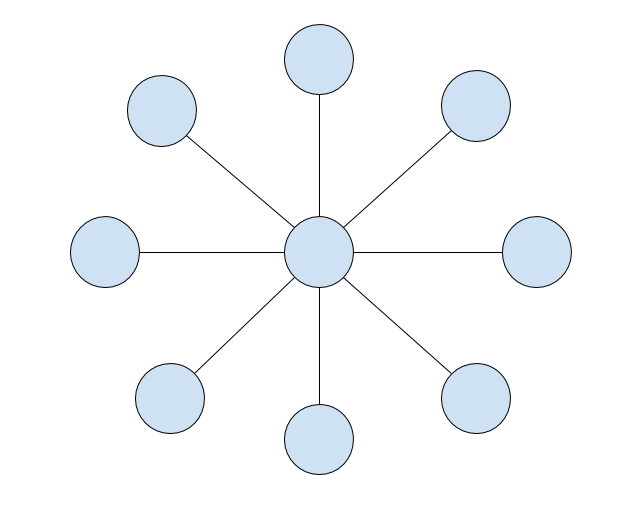
\includegraphics[scale=0.25]{img/spokes.png}
        \end{column}
    \end{columns}
\end{frame}
%%%%%%%%%%%%%%%%%%%%%%%%%%%%%%%%%%%%%%%%%%%%%%%%%%%%%%%%%%%%%%%%%%%%%%%%%%%%%%%
\begin{frame}[fragile] \frametitle{}
    \slideheader{Multivariate Gaussian}
\end{frame}
%%%%%%%%%%%%%%%%%%%%%%%%%%%%%%%%%%%%%%%%%%%%%%%%%%%%%%%%%%%%%%%%%%%%%%%%%%%%%%%
% Pairwise Recovery
%%%%%%%%%%%%%%%%%%%%%%%%%%%%%%%%%%%%%%%%%%%%%%%%%%%%%%%%%%%%%%%%%%%%%%%%%%%%%%%
\begin{frame}[fragile] \frametitle{}
    \sectionslide{Precision Matrix Estimation}
\end{frame}
%%%%%%%%%%%%%%%%%%%%%%%%%%%%%%%%%%%%%%%%%%%%%%%%%%%%%%%%%%%%%%%%%%%%%%%%%%%%%%%
\begin{frame}[fragile] \frametitle{}
    \slideheader{Maximum Likelihood Estimation}
\end{frame}
%%%%%%%%%%%%%%%%%%%%%%%%%%%%%%%%%%%%%%%%%%%%%%%%%%%%%%%%%%%%%%%%%%%%%%%%%%%%%%%
\begin{frame}[fragile] \frametitle{}
    \slideheader{Maximum Likelihood Estimation: Issues}
\end{frame}
%%%%%%%%%%%%%%%%%%%%%%%%%%%%%%%%%%%%%%%%%%%%%%%%%%%%%%%%%%%%%%%%%%%%%%%%%%%%%%%
\begin{frame}[fragile] \frametitle{}
    \slideheader{Graphical Lasso}
\end{frame}
%%%%%%%%%%%%%%%%%%%%%%%%%%%%%%%%%%%%%%%%%%%%%%%%%%%%%%%%%%%%%%%%%%%%%%%%%%%%%%%
\begin{frame}[fragile] \frametitle{}
    \slideheader{Asymptotic Normal Thresholding (ANT)}
\end{frame}
%%%%%%%%%%%%%%%%%%%%%%%%%%%%%%%%%%%%%%%%%%%%%%%%%%%%%%%%%%%%%%%%%%%%%%%%%%%%%%%
% Risk Bounds
%%%%%%%%%%%%%%%%%%%%%%%%%%%%%%%%%%%%%%%%%%%%%%%%%%%%%%%%%%%%%%%%%%%%%%%%%%%%%%%
\begin{frame}[fragile] \frametitle{}
    \sectionslide{Risk Bounds in $\norm{\cdot}_\infty$}
\end{frame}
%%%%%%%%%%%%%%%%%%%%%%%%%%%%%%%%%%%%%%%%%%%%%%%%%%%%%%%%%%%%%%%%%%%%%%%%%%%%%%%
\begin{frame}[fragile] \frametitle{}
    \slideheader{Risk Upper Bound}

    \theorem{Lorem ipsum.}

\end{frame}
%%%%%%%%%%%%%%%%%%%%%%%%%%%%%%%%%%%%%%%%%%%%%%%%%%%%%%%%%%%%%%%%%%%%%%%%%%%%%%%
\begin{frame}[fragile] \frametitle{}
    \slideheader{Oracle Inequalities}
\end{frame}
%%%%%%%%%%%%%%%%%%%%%%%%%%%%%%%%%%%%%%%%%%%%%%%%%%%%%%%%%%%%%%%%%%%%%%%%%%%%%%%
\begin{frame}[fragile] \frametitle{}
    \slideheader{Coupling Argument}
\end{frame}
%%%%%%%%%%%%%%%%%%%%%%%%%%%%%%%%%%%%%%%%%%%%%%%%%%%%%%%%%%%%%%%%%%%%%%%%%%%%%%%
\begin{frame}[fragile] \frametitle{}
    \slideheader{Risk Lower Bound}
\end{frame}
%%%%%%%%%%%%%%%%%%%%%%%%%%%%%%%%%%%%%%%%%%%%%%%%%%%%%%%%%%%%%%%%%%%%%%%%%%%%%%%
\begin{frame}[fragile] \frametitle{}
    \slideheader{Le Cam's Two-Point Argument}
\end{frame}
%%%%%%%%%%%%%%%%%%%%%%%%%%%%%%%%%%%%%%%%%%%%%%%%%%%%%%%%%%%%%%%%%%%%%%%%%%%%%%%
\begin{frame}[fragile] \frametitle{}
    \sectionslide{Next Steps}
\end{frame}
%%%%%%%%%%%%%%%%%%%%%%%%%%%%%%%%%%%%%%%%%%%%%%%%%%%%%%%%%%%%%%%%%%%%%%%%%%%%%%%
\end{document}

